\documentclass{article}
\usepackage{oconnor}
\usepackage{ wasysym }

%% UPDATE these variables:
\renewcommand{\hwnum}{6}
\title{CSCI 338, Quiz 06}
\author{Patrick O'Connor}
\collab{n/a}
%%\date{due: 15 January 2021}

\begin{document}

\maketitle

CSCI 338 Computer Science Theory
1 (3 points; due: 10am, May 20)
This is a quiz (not an attendance counting), so you should 
try your best.Note also that this is an open book quiz, 
while all physical resources are allowed, resorting for external human 
help constitutes aplagiarism


% ============================================
% ============================================
\nextprob{Question 1}
\collab{n/a}
% ============================================
Using pumping lemma to prove that the following language is not context-free.

$L = \{a^n b^j c^k$ $|$ $k=nj\}$.

\paragraph{Answer}

Please see figure \ref{fig:num01}
\begin{figure}
    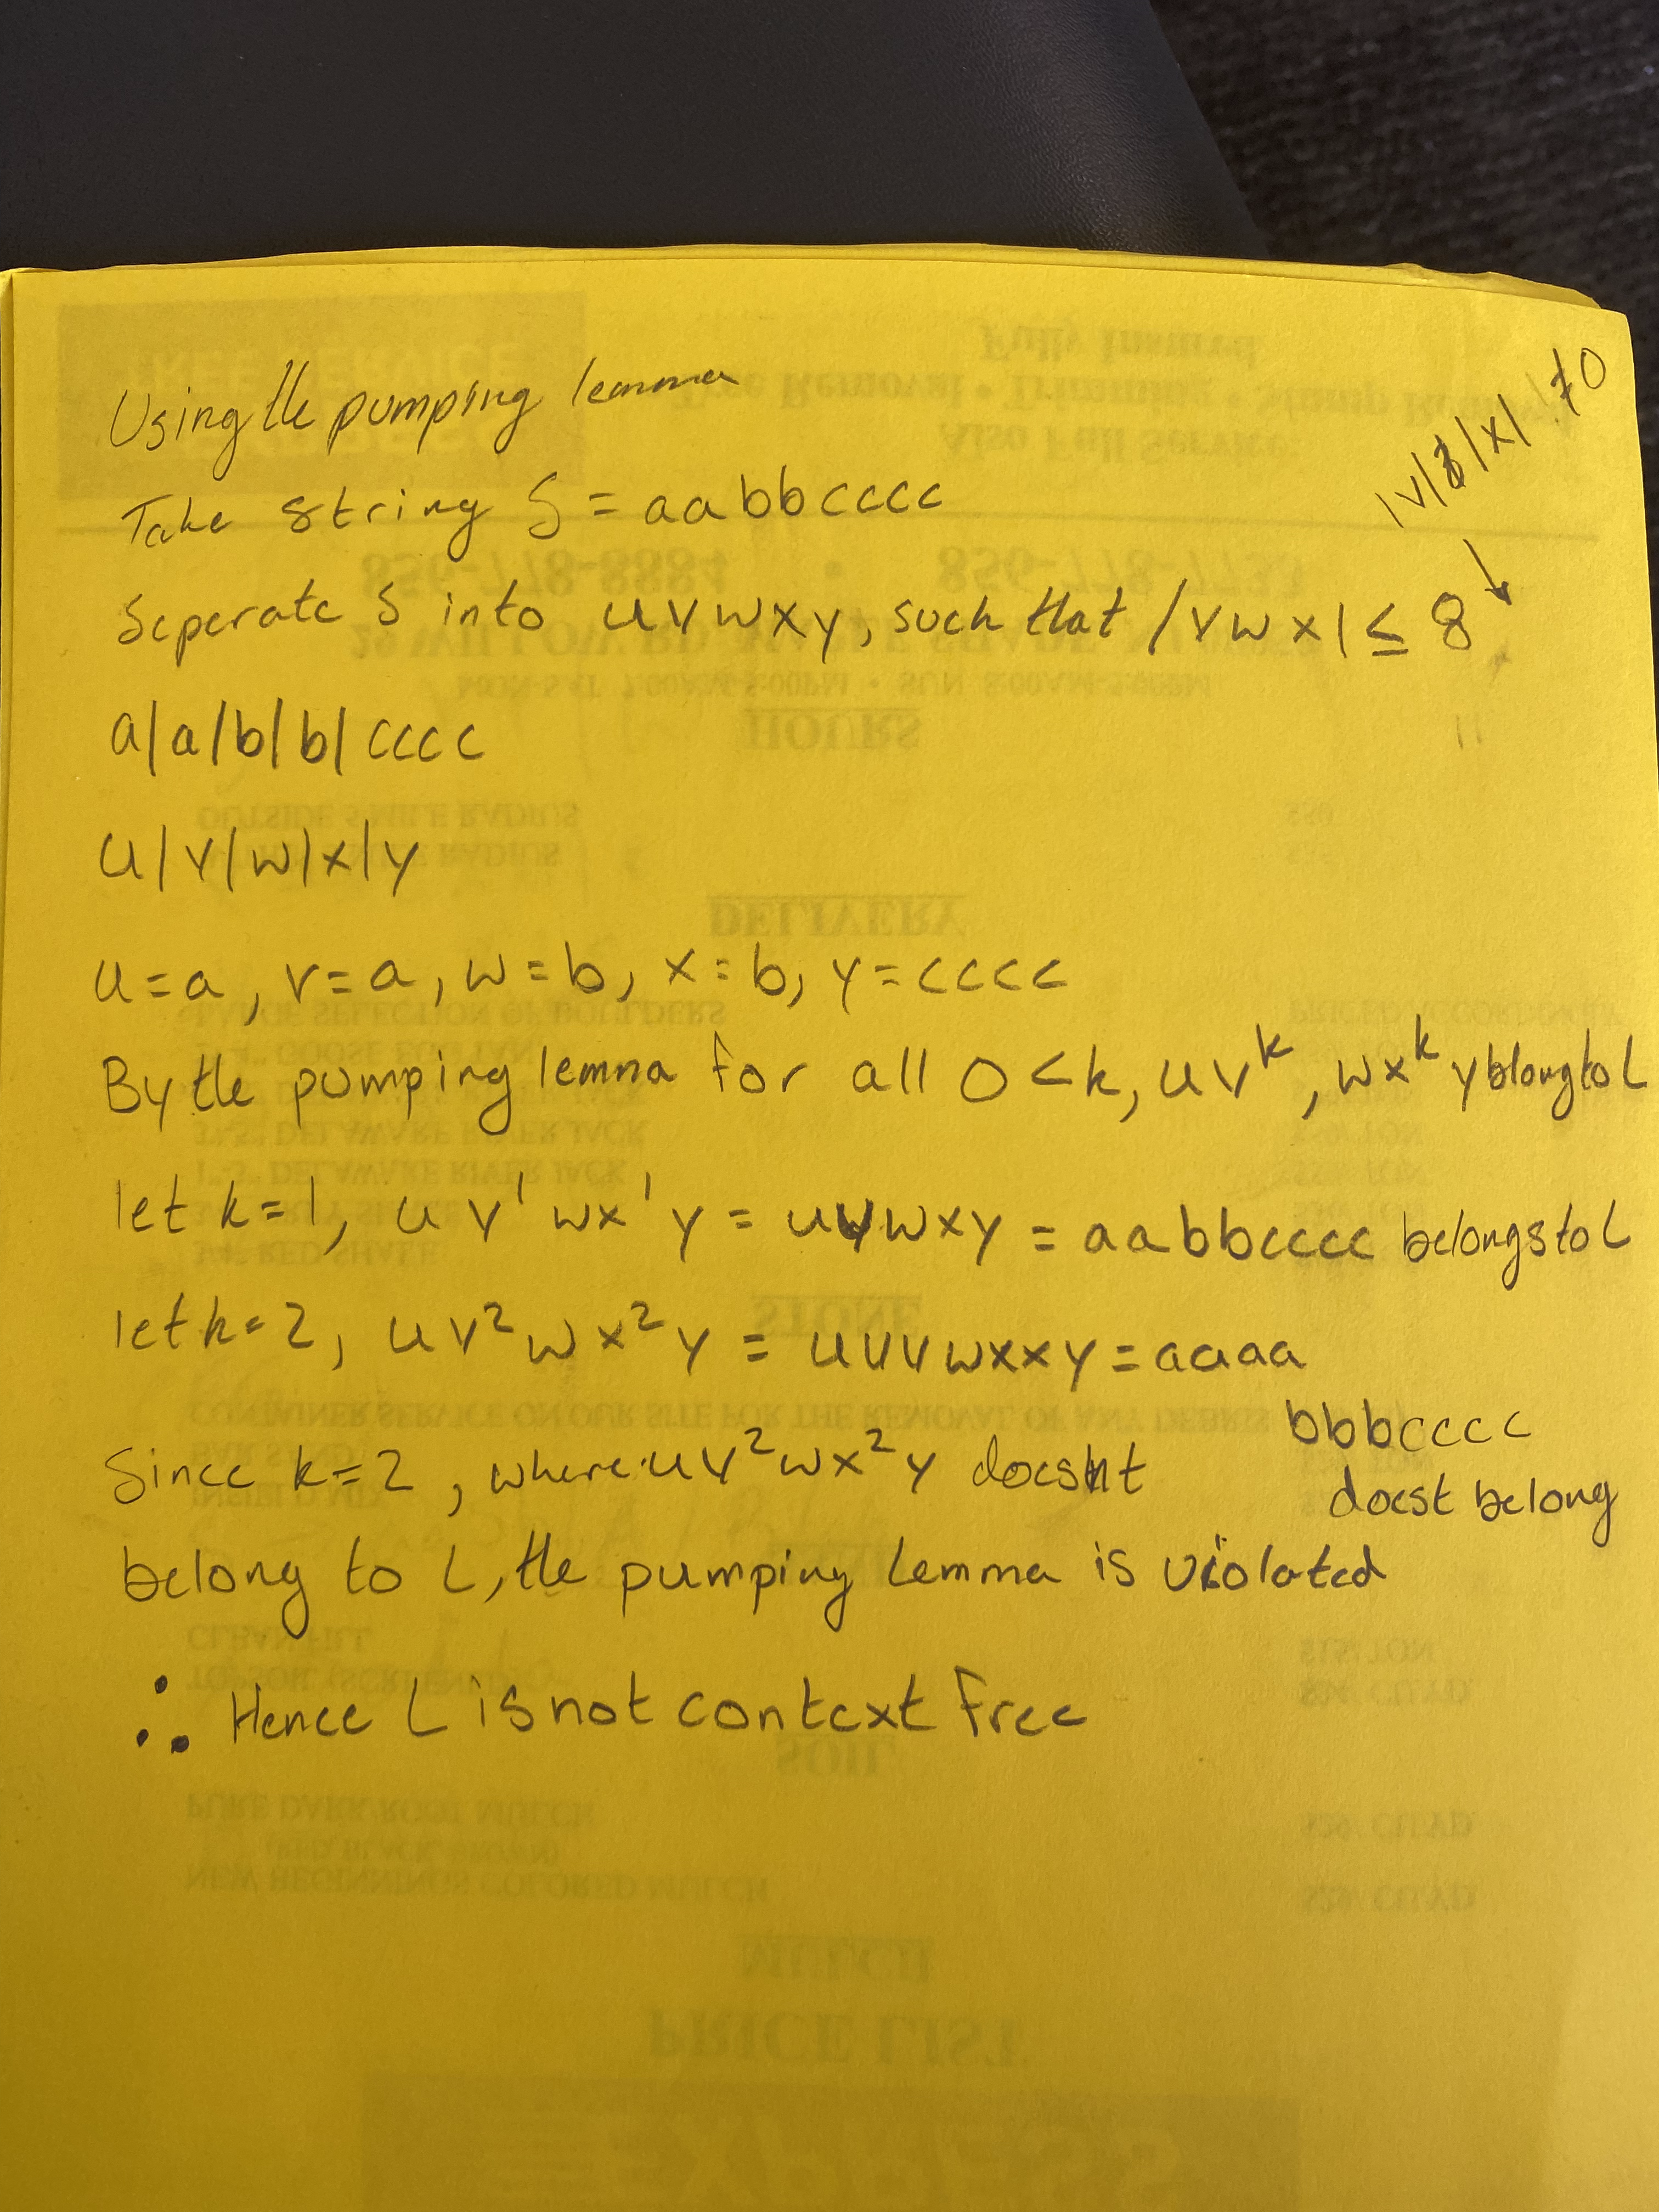
\includegraphics[width=\linewidth]{01.png}
    \caption{Language L is not context-free}
    \label{fig:num01}
\end{figure}

\end{document}

